%% bare_jrnl.tex
%% V1.4b
%% 2015/08/26
%% by Michael Shell
%% see http://www.michaelshell.org/
%% for current contact information.
%%
%% This is a skeleton file demonstrating the use of IEEEtran.cls
%% (requires IEEEtran.cls version 1.8b or later) with an IEEE
%% journal paper.
%%
%% Support sites:
%% http://www.michaelshell.org/tex/ieeetran/
%% http://www.ctan.org/pkg/ieeetran
%% and
%% http://www.ieee.org/

%%*************************************************************************
%% Legal Notice:
%% This code is offered as-is without any warranty either expressed or
%% implied; without even the implied warranty of MERCHANTABILITY or
%% FITNESS FOR A PARTICULAR PURPOSE! 
%% User assumes all risk.
%% In no event shall the IEEE or any contributor to this code be liable for
%% any damages or losses, including, but not limited to, incidental,
%% consequential, or any other damages, resulting from the use or misuse
%% of any information contained here.
%%
%% All comments are the opinions of their respective authors and are not
%% necessarily endorsed by the IEEE.
%%
%% This work is distributed under the LaTeX Project Public License (LPPL)
%% ( http://www.latex-project.org/ ) version 1.3, and may be freely used,
%% distributed and modified. A copy of the LPPL, version 1.3, is included
%% in the base LaTeX documentation of all distributions of LaTeX released
%% 2003/12/01 or later.
%% Retain all contribution notices and credits.
%% ** Modified files should be clearly indicated as such, including  **
%% ** renaming them and changing author support contact information. **
%%*************************************************************************


% *** Authors should verify (and, if needed, correct) their LaTeX system  ***
% *** with the testflow diagnostic prior to trusting their LaTeX platform ***
% *** with production work. The IEEE's font choices and paper sizes can   ***
% *** trigger bugs that do not appear when using other class files.       ***                          ***
% The testflow support page is at:
% http://www.michaelshell.org/tex/testflow/



\documentclass[journal]{IEEEtran}
%
% If IEEEtran.cls has not been installed into the LaTeX system files,
% manually specify the path to it like:
% \documentclass[journal]{../sty/IEEEtran}

%**** LANGUAGE PACKAGES *****



% Some very useful LaTeX packages include:
% (uncomment the ones you want to load)


% *** MISC UTILITY PACKAGES ***
%
%\usepackage{ifpdf}
% Heiko Oberdiek's ifpdf.sty is very useful if you need conditional
% compilation based on whether the output is pdf or dvi.
% usage:
% \ifpdf
%   % pdf code
% \else
%   % dvi code
% \fi
% The latest version of ifpdf.sty can be obtained from:
% http://www.ctan.org/pkg/ifpdf
% Also, note that IEEEtran.cls V1.7 and later provides a builtin
% \ifCLASSINFOpdf conditional that works the same way.
% When switching from latex to pdflatex and vice-versa, the compiler may
% have to be run twice to clear warning/error messages.



% *** CITATION PACKAGES ***
%
\usepackage{cite}
% cite.sty was written by Donald Arseneau
% V1.6 and later of IEEEtran pre-defines the format of the cite.sty package
% \cite{} output to follow that of the IEEE. Loading the cite package will
% result in citation numbers being automatically sorted and properly
% "compressed/ranged". e.g., [1], [9], [2], [7], [5], [6] without using
% cite.sty will become [1], [2], [5]--[7], [9] using cite.sty. cite.sty's
% \cite will automatically add leading space, if needed. Use cite.sty's
% noadjust option (cite.sty V3.8 and later) if you want to turn this off
% such as if a citation ever needs to be enclosed in parenthesis.
% cite.sty is already installed on most LaTeX systems. Be sure and use
% version 5.0 (2009-03-20) and later if using hyperref.sty.
% The latest version can be obtained at:
% http://www.ctan.org/pkg/cite
% The documentation is contained in the cite.sty file itself.


% *** GRAPHICS RELATED PACKAGES ***
%
\ifCLASSINFOpdf
 \usepackage[pdftex]{graphicx}
 \usepackage{subfigure} % subfiguras
  % declare the path(s) where your graphic files are 
 \graphicspath{ {images/} }
  % and their extensions so you won't have to specify these with
  % every instance of \includegraphics
  \DeclareGraphicsExtensions{.pdf,.jpeg,.png}
\else
  % or other class option (dvipsone, dvipdf, if not using dvips). graphicx
  % will default to the driver specified in the system graphics.cfg if no
  % driver is specified.
  % \usepackage[dvips]{graphicx}
  % declare the path(s) where your graphic files are
  % \graphicspath{{../eps/}}
  % and their extensions so you won't have to specify these with
  % every instance of \includegraphics
  % \DeclareGraphicsExtensions{.eps}
\fi
% graphicx was written by David Carlisle and Sebastian Rahtz. It is
% required if you want graphics, photos, etc. graphicx.sty is already
% installed on most LaTeX systems. The latest version and documentation
% can be obtained at: 
% http://www.ctan.org/pkg/graphicx
% Another good source of documentation is "Using Imported Graphics in
% LaTeX2e" by Keith Reckdahl which can be found at:
% http://www.ctan.org/pkg/epslatex
%
% latex, and pdflatex in dvi mode, support graphics in encapsulated
% postscript (.eps) format. pdflatex in pdf mode supports graphics
% in .pdf, .jpeg, .png and .mps (metapost) formats. Users should ensure
% that all non-photo figures use a vector format (.eps, .pdf, .mps) and
% not a bitmapped formats (.jpeg, .png). The IEEE frowns on bitmapped formats
% which can result in "jaggedy"/blurry rendering of lines and letters as
% well as large increases in file sizes.
%
% You can find documentation about the pdfTeX application at:
% http://www.tug.org/applications/pdftex




% *** MATH PACKAGES ***
%
\usepackage{amsmath}
% A popular package from the American Mathematical Society that provides
% many useful and powerful commands for dealing with mathematics.
%
% Note that the amsmath package sets \interdisplaylinepenalty to 10000
% thus preventing page breaks from occurring within multiline equations. Use:
%\interdisplaylinepenalty=2500
% after loading amsmath to restore such page breaks as IEEEtran.cls normally
% does. amsmath.sty is already installed on most LaTeX systems. The latest
% version and documentation can be obtained at:
% http://www.ctan.org/pkg/amsmath



% *** SPECIALIZED LIST PACKAGES ***
%
\usepackage{algorithmic}
% algorithmic.sty was written by Peter Williams and Rogerio Brito.
% This package provides an algorithmic environment fo describing algorithms.
% You can use the algorithmic environment in-text or within a figure
% environment to provide for a floating algorithm. Do NOT use the algorithm
% floating environment provided by algorithm.sty (by the same authors) or
% algorithm2e.sty (by Christophe Fiorio) as the IEEE does not use dedicated
% algorithm float types and packages that provide these will not provide
% correct IEEE style captions. The latest version and documentation of
% algorithmic.sty can be obtained at:
% http://www.ctan.org/pkg/algorithms
% Also of interest may be the (relatively newer and more customizable)
% algorithmicx.sty package by Szasz Janos:
% http://www.ctan.org/pkg/algorithmicx



\usepackage{xspace} 

% *** ALIGNMENT PACKAGES ***
%
\usepackage{array}
% Frank Mittelbach's and David Carlisle's array.sty patches and improves
% the standard LaTeX2e array and tabular environments to provide better
% appearance and additional user controls. As the default LaTeX2e table
% generation code is lacking to the point of almost being broken with
% respect to the quality of the end results, all users are strongly
% advised to use an enhanced (at the very least that provided by array.sty)
% set of table tools. array.sty is already installed on most systems. The
% latest version and documentation can be obtained at:
% http://www.ctan.org/pkg/array


% IEEEtran contains the IEEEeqnarray family of commands that can be used to
% generate multiline equations as well as matrices, tables, etc., of high
% quality.




% *** SUBFIGURE PACKAGES ***
%\ifCLASSOPTIONcompsoc
%  \usepackage[caption=false,font=normalsize,labelfont=sf,textfont=sf]{subfig}
%\else
%  \usepackage[caption=false,font=footnotesize]{subfig}
%\fi
% subfig.sty, written by Steven Douglas Cochran, is the modern replacement
% for subfigure.sty, the latter of which is no longer maintained and is
% incompatible with some LaTeX packages including fixltx2e. However,
% subfig.sty requires and automatically loads Axel Sommerfeldt's caption.sty
% which will override IEEEtran.cls' handling of captions and this will result
% in non-IEEE style figure/table captions. To prevent this problem, be sure
% and invoke subfig.sty's "caption=false" package option (available since
% subfig.sty version 1.3, 2005/06/28) as this is will preserve IEEEtran.cls
% handling of captions.
% Note that the Computer Society format requires a larger sans serif font
% than the serif footnote size font used in traditional IEEE formatting
% and thus the need to invoke different subfig.sty package options depending
% on whether compsoc mode has been enabled.
%
% The latest version and documentation of subfig.sty can be obtained at:
% http://www.ctan.org/pkg/subfig




% *** FLOAT PACKAGES ***
%
%\usepackage{fixltx2e}
% fixltx2e, the successor to the earlier fix2col.sty, was written by
% Frank Mittelbach and David Carlisle. This package corrects a few problems
% in the LaTeX2e kernel, the most notable of which is that in current
% LaTeX2e releases, the ordering of single and double column floats is not
% guaranteed to be preserved. Thus, an unpatched LaTeX2e can allow a
% single column figure to be placed prior to an earlier double column
% figure.
% Be aware that LaTeX2e kernels dated 2015 and later have fixltx2e.sty's
% corrections already built into the system in which case a warning will
% be issued if an attempt is made to load fixltx2e.sty as it is no longer
% needed.
% The latest version and documentation can be found at:
% http://www.ctan.org/pkg/fixltx2e


%\usepackage{stfloats}
% stfloats.sty was written by Sigitas Tolusis. This package gives LaTeX2e
% the ability to do double column floats at the bottom of the page as well
% as the top. (e.g., "\begin{figure*}[!b]" is not normally possible in
% LaTeX2e). It also provides a command:
%\fnbelowfloat
% to enable the placement of footnotes below bottom floats (the standard
% LaTeX2e kernel puts them above bottom floats). This is an invasive package
% which rewrites many portions of the LaTeX2e float routines. It may not work
% with other packages that modify the LaTeX2e float routines. The latest
% version and documentation can be obtained at:
% http://www.ctan.org/pkg/stfloats
% Do not use the stfloats baselinefloat ability as the IEEE does not allow
% \baselineskip to stretch. Authors submitting work to the IEEE should note
% that the IEEE rarely uses double column equations and that authors should try
% to avoid such use. Do not be tempted to use the cuted.sty or midfloat.sty
% packages (also by Sigitas Tolusis) as the IEEE does not format its papers in
% such ways.
% Do not attempt to use stfloats with fixltx2e as they are incompatible.
% Instead, use Morten Hogholm'a dblfloatfix which combines the features
% of both fixltx2e and stfloats:
%
% \usepackage{dblfloatfix}
% The latest version can be found at:
% http://www.ctan.org/pkg/dblfloatfix




%\ifCLASSOPTIONcaptionsoff
%  \usepackage[nomarkers]{endfloat}
% \let\MYoriglatexcaption\caption
% \renewcommand{\caption}[2][\relax]{\MYoriglatexcaption[#2]{#2}}
%\fi
% endfloat.sty was written by James Darrell McCauley, Jeff Goldberg and 
% Axel Sommerfeldt. This package may be useful when used in conjunction with 
% IEEEtran.cls'  captionsoff option. Some IEEE journals/societies require that
% submissions have lists of figures/tables at the end of the paper and that
% figures/tables without any captions are placed on a page by themselves at
% the end of the document. If needed, the draftcls IEEEtran class option or
% \CLASSINPUTbaselinestretch interface can be used to increase the line
% spacing as well. Be sure and use the nomarkers option of endfloat to
% prevent endfloat from "marking" where the figures would have been placed
% in the text. The two hack lines of code above are a slight modification of
% that suggested by in the endfloat docs (section 8.4.1) to ensure that
% the full captions always appear in the list of figures/tables - even if
% the user used the short optional argument of \caption[]{}.
% IEEE papers do not typically make use of \caption[]'s optional argument,
% so this should not be an issue. A similar trick can be used to disable
% captions of packages such as subfig.sty that lack options to turn off
% the subcaptions:
% For subfig.sty:
% \let\MYorigsubfloat\subfloat
% \renewcommand{\subfloat}[2][\relax]{\MYorigsubfloat[]{#2}}
% However, the above trick will not work if both optional arguments of
% the \subfloat command are used. Furthermore, there needs to be a
% description of each subfigure *somewhere* and endfloat does not add
% subfigure captions to its list of figures. Thus, the best approach is to
% avoid the use of subfigure captions (many IEEE journals avoid them anyway)
% and instead reference/explain all the subfigures within the main caption.
% The latest version of endfloat.sty and its documentation can obtained at:
% http://www.ctan.org/pkg/endfloat
%
% The IEEEtran \ifCLASSOPTIONcaptionsoff conditional can also be used
% later in the document, say, to conditionally put the References on a 
% page by themselves.




% *** PDF, URL AND HYPERLINK PACKAGES ***
%
%\usepackage{url}
% url.sty was written by Donald Arseneau. It provides better support for
% handling and breaking URLs. url.sty is already installed on most LaTeX
% systems. The latest version and documentation can be obtained at:
% http://www.ctan.org/pkg/url
% Basically, \url{my_url_here}.


\usepackage{authblk}

% *** Do not adjust lengths that control margins, column widths, etc. ***
% *** Do not use packages that alter fonts (such as pslatex).         ***
% There should be no need to do such things with IEEEtran.cls V1.6 and later.
% (Unless specifically asked to do so by the journal or conference you plan
% to submit to, of course. )


% correct bad hyphenation here
\hyphenation{op-tical net-works semi-conduc-tor}

% Paquete para saltos del inea
\usepackage[utf8]{inputenc}


% Paquete para utilizar colores
\usepackage{color}

% **** PLOTS PACKAGE ************
\usepackage{pgfplots}

\begin{document}
%
% paper title
% Titles are generally capitalized except for words such as a, an, and, %as,
% at, but, by, for, in, nor, of, on, or, the, to and up, which are usually
% not capitalized unless they are the first or last word of the title.
% Linebreaks \\ can be used within to get better formatting as desired.
% Do not put math or special symbols in the title.
\title{ Power-Efficient Model of Blockchain Applications in Mobile Systems }
%
%
% author names and IEEE memberships
% note positions of commas and nonbreaking spaces ( ~ ) LaTeX will not break
% a structure at a ~ so this keeps an author's name from being broken across
% two lines.
% use \thanks{} to gain access to the first footnote area
% a separate \thanks must be used for each paragraph as LaTeX2e's \thanks
% was not built to handle multiple paragraphs
%

\author{Manuel Figueroa,\IEEEmembership{ ITCR,}
        Esteban Leandro,\IEEEmembership{ ITCR}}% <-this % stops a space
\affil[]{\textit{MC-7201 Introduction to Research}}
\affil[]{\textit{Instituto Tecnológico de Costa Rica}}
\affil[]{\textit{\{mfigueroacr, elc790\}@gmail.com}}

% note the % following the last \IEEEmembership and also \thanks - 
% these prevent an unwanted space from occurring between the last author name
% and the end of the author line. i.e., if you had this:
% 
% \author{....lastname \thanks{...} \thanks{...} }
%                     ^------------^------------^----Do not want these spaces!
%
% a space would be appended to the last name and could cause every name on that
% line to be shifted left slightly. This is one of those "LaTeX things". For
% instance, "\textbf{A} \textbf{B}" will typeset as "A B" not "AB". To get
% "AB" then you have to do: "\textbf{A}\textbf{B}"
% \thanks is no different in this regard, so shield the last } of each \thanks
% that ends a line with a % and do not let a space in before the next \thanks.
% Spaces after \IEEEmembership other than the last one are OK (and needed) as
% you are supposed to have spaces between the names. For what it is worth,
% this is a minor point as most people would not even notice if the said evil
% space somehow managed to creep in.



% The paper headers
\markboth{ININ Power Modeling of blockchain applications in mobile systems, 2019}%
{Shell \MakeLowercase{\textit{et al.}}: Power modeling of blockchain applications in mobile systems }
% The only time the second header will appear is for the odd numbered pages
% after the title page when using the twoside option.
% 
% *** Note that you probably will NOT want to include the author's ***
% *** name in the headers of peer review papers.                   ***
% You can use \ifCLASSOPTIONpeerreview for conditional compilation here if
% you desire.




% If you want to put a publisher's ID mark on the page you can do it like
% this:
%\IEEEpubid{0000--0000/00\$00.00~\copyright~2015 IEEE}
% Remember, if you use this you must call \IEEEpubidadjcol in the second
% column for its text to clear the IEEEpubid mark.



% use for special paper notices
%\IEEEspecialpapernotice{(Invited Paper)}




% make the title area
\maketitle

% As a general rule, do not put math, special symbols or citations
% in the abstract or keywords.
\begin{abstract}
  Since security has become a major concern in the everyday use of technology. 
  The impact of mobiles and the growing dependency that the general population has in mobile devices and systems has
  increased its potentially harmful impact of a security breach. Most of the interaction between users with systems,
  including banking and e-commerce are made using mobile devices. Recently the introduction of the blockchain technology
  as an effective security solution for many applications that involve transactions, 
  also as hardware evolves those mobile devices now have larger processing capabilities that make it possible 
  to run blockchain based solution in the mobile space. A definition of a power model allow us to describe, 
  understand and predict the expected behavior of the power consumption demand in those kind of solutions and will
  help the system designers to estimate how the devices will behave in terms of power consumption.
  Also, it will help application designers to define the scope of its application in terms of performance and power 
  consumption when it is executed in a mobile device and a high compute rate is expected to perform the blockchain mining process.
\end{abstract}

% Note that keywords are not normally used for peerreview papers.
\begin{IEEEkeywords}
\LaTeX\xspace mobile systems, blockchain, power modeling.
\end{IEEEkeywords}






% For peer review papers, you can put extra information on the cover
% page as needed:
% \ifCLASSOPTIONpeerreview
% \begin{center} \bfseries EDICS Category: 3-BBND \end{center}
% \fi
%
% For peerreview papers, this IEEEtran command inserts a page break and
% creates the second title. It will be ignored for other modes.
\IEEEpeerreviewmaketitle



\section{Introduction}
\subsection{Blockchain}
Blockchain has been introduced in the last years as a technology method for data security problems, where there are several implementations of it, like Bitcoin Wallet \cite{Bamert2017}, Ripples or Ethereum\cite{Buterin2017}, as many others crypto currencies. 

Besides that, deleting the intermediary from the equation through a bank transaction between an account to another and giving that control to the users has been an interesting approach, where there is a big pool of users that approve those transactions if those are valid to be added to the block chain, with the difference that nobody knows which is the origin user and the destination user, the inly information needed is that a virtual wallet is sending some money or crypto currency to another wallet identified by an address.

After a transaction is created is grouped into blocks, and the links between blocks and their content are protected by cryptography and cannot be forged. Once that the transaction is inside the blockchain, there is no way to erase it.

\subsection{Mining}
Kroll et al. \cite{Kroll2013} explain that the mining process requires vast computing power as only a "brute force, trial and error" method can be used to calculate the SHA-256 hash. Every two weeks, the complexity of the challenge is adjusted to ensure that, on average, a block is mined every 10 minutes. The financial incentive of 25 bitcoins is offered to the first miner to successfully calculate the hash. 

This technique may lead money earnings but also requires alot of computing resources consuming, as electricity, also this technical hardware and software equipment is not available in every country, sometimes there is a cost of buy in them when the mining team is in a place that makes them get it from exterior. But worth to mention it as part of the whole blockchain and crypto currencies possibilities.

\subsection{Blockchain and Internet of Things}
This concept adapts to the blockchain and mobile relation, as there are daily millions and millions of devices moving transactions from one side to another, using bank accounts or orher payment methods which may several waits from clients, time consuming and more. Millions of mobile devices can avoid the bank intermediary by handling their transactions inside the blockchain.

As stuff and not just people are related with the Internet every day, blockchain is a very advanced technique to interconnect transaction systems, as monitoring systems, health, finance, education and more.

Modern Internet of Things(IoT) software systems, like interconnected transportation systems, generate a lot if data every day. The data exchanges may charge a fee for handeling the transactions inside the wallets, which may also elevate costs, security concerns and privacy of several transactions for a single entity \cite{TQiu2017}. 

\subsection{Contribution}
In this paper, we describe a new algorithm that enable any kind of mobile devices, including Android and iOS mobile operating systems, to run transaction applications with several amounts of traffic (our tests are based on two hundred transactions per second), where the mobile device can handle that amount of traffic and keep the user interface without lacks or interrumptions to the user. The 70 percentage of the transactions used to test the algorithm were on devices with Linux based operating systems.

All transactions used in this experiment used non bank accounts between source and destination accounts, but blockchain in order to add every transaction to the chain where will be approved by other users. 

The performance shown is superior than bank systems in 30 percentage as the experiments show. We think this is part because the bank software systems sometimes are old, or even new sometimes data need to be moved from one side to another using cronjobs or tasks schedulers which is not in real time.

Our approach avoids all this waiting times, given an algorithm which can be used in several markets that includes monetary transactions, via your cellphone or anu mobile device.


\section{Background}
\subsection{Mobile Blockchain Systems}
According to \cite{crosby2016} a blockchain system can be seen as a distributed database of records. 
The system provides a public layer that keeps a record for every single event that have been executed among the participant parties.
Each new transaction added to the blockchain requires a process to be included as a new block in the blockchain. That process requires some kind of validation, usually
solving a proof-of-work puzzle.
That kind of implementation is expensive and it has been hard to include a proper blockchain system in mobile architectures
due to the lack of computing power and the limited energy of current mobile devices. For that reason some other approaches \cite{xiongfengniyatowanghan2018}, \cite{ZehuiXiong} have been studied to enable
blockchain application to be used in the mobile devices. 
In those approaches, the authors claim that is a good idea to offload the mining process to an edge computing service provider, this will eventually enable any 
device to participate as an active node in the blockchain network even if they are no capable of performing any mining process at all. 
In that scenario the network must be supported by an external service and that will reduce the \emph{free-network} concept. The mobile devices will participate  as dumb clients and the entire
blockchain process will be performed in the cloud.
Also this novel approach and will be excellent to support e-commerce initiatives and will not limit the participation of
users due to lack of computational power.

\subsection{Power Monitoring}
According to \cite{fairley2017} the bitcoin miners are considered electromagnetic alchemist, because they can convert massive amounts of megawatt-hours of electricity into the world's fastest-growing currency.
Because of the calculations required to hash a transaction block and correctly include it in the chain it is estimate that a bitcoin transaction consumes more than 5,000 times as much energy as using a Visa credit card.
Even when the computers are constantly getting faster and more power efficient, the bitcoin algorithm increase the difficulty of the hashing procedures to keep the chain integrity and security by making almost impossible to introduce malicious blocks by outrunning the entire network and producing a new longer chain with the fraudulent blocks. That causes a huge impact in the power consumption of the platform, and it is estimates in a total of 73.12 TWh or the same as the entire consumption of Austria \cite{digiconomist}.

Actually some strategies are implemented to solve this amount of power required to include a new block 
in the blockchain, some of them are related to change the proof-of-work algorithm to something more power
 efficient like Algorand \cite{giladhemomicalivlachoszeldovich2017}, using the Bizantine agreements technique to reach consensus, and others like proof-of-learning \cite{bravo-marquezreevesugarte2019} that use rankings of machine learning systems.

It is possible to measure the power consumption of a component using the Ohm's law that will express a value in \emph{Watts} and can be expressed as the following equation: 
\begin{center}
    $Power(Watts) = V * I$
\end{center}
where V is the volatage given in \emph{Volts} and I is the current given in \emph{Amperes}. We can use performance monitoring counters (PFC) \cite{perfmonitoring:1991} to measure the amount of power required by a blockchain network with local nodes, and therefore estimate the total amount of power required when it scales up.

To the best of our knowledge there is no a commercial implementation of a blockchain system running on mobile devices, perhaps an hybrid scheme would be feasible, and the MobiChain \cite{Suankaewmanee} is an approach that can run the mining process using mobile nodes. 

It is part of our interest to know what is the power modeling of a mobile blockchain system using other consensus mechanisms and verify if that would make them and attractive  option to be incorporated in mobile e-commerce platforms.




\section{Implementation}

\subsection{Algorithm Explanation}
The main advantage of our algorithm implementation is to use a different way to perform the proof-of-work blocks validation, since that is the part that requires the larger amount of time to be performed and also the larger amount of consumed power due to the difficult mathematical puzzle to be performed by the participant nodes.

Our approach consists in to implement the blockchain validation using a bizantine agreement approach proposed by \cite{giladhemomicalivlachoszeldovich2017} using a similar proof-of-stake approach. According to that implementation the power of mining is given by the amount of tokens that the participant has in the system. A peer with more tokens has the major possibility of getting a new block added to the system, and it is based in the supposition that the peer with the larger amount of tokens is interested in keeping the security of the whole platform in good shape.

Since the amount of required computing power to perform those bizantine agreements is considerably lower than the proof-of-work then we can presume that the expected performance will be higher than the algorithm proposed by \cite{Suankaewmanee} and also with a lower power consumption requirements.


\subsection{Experiments}
All of our experiments will be performed using a set of  5 Kindle Fire 10, with a 1.2GHz quad-core processor, and 1GB RAM, and a set pf 5 Samsung Galaxy S5 with a 2.5 GHz quad-core processor and Qualcomm Adreno 330 GPU with 450Mhz core processor and 2GB RAM.

We choose those devieces because they represent the average specs of a current date smartphone, and since the mobile devices increase its computational power every year we can also expect that results will be better in the future.

In our experiment, we create a blockchain of 8000 blocks and use the mentioned set of mobile devices to mine thee block.

The expected result of the algorithm is to mine that chain of blocks under 3 days of time to beat the time presented by MobiChain in \cite{Suankaewmanee}. 

\subsection{Results}

In this section we show the expected results of the exection of our algorithm processing a set of 8000 blocks using a combined network of mobile devices as descripted above.

The following table shows the amount of time (in seconds) expected by the network to complete a block chain of certain number of blocks. The amount of Kindle devices used is represented by \emph{\#K} and the amount of Samsung devices is represented by \emph{\#S} 

\begin{table}[h!] 
\begin{center} 
\begin{tabular}{|l|c|c|c|}
%\begin{tabular}%{|m{2cm}|m{1.5cm}|m{1.5cm}|m{1.5cm}|}
\hline 

\textbf{\# Blocks} & \textbf{4 Nodes} & \textbf{8 Nodes}  & \textbf{10 Nodes}  \\ 
\textbf{}& \textbf{2 K + 2S} & \textbf{4K + 4S} & \textbf{5K + 5S} \\
\hline 
2000 & 25 & 23 & 18.5\\ 
\hline 
4000 & 45 & 42.1 & 38.43\\ 
\hline 
6000 & 83.8 & 81 & 76.25 \\ 
\hline 
8000 & 120 & 110 & 106 \\
\hline 

\end{tabular} 
\end{center} 
\caption{Blockchain Creation Time} 
\end{table}

The results presented here are estimated using 3 cores per node and equal number of threads per core by calculate the validation proof of every block prior add them to the chain. The network latency will not be considered since every node in this experiment are under the same network using a 1Gb/s speed connection.

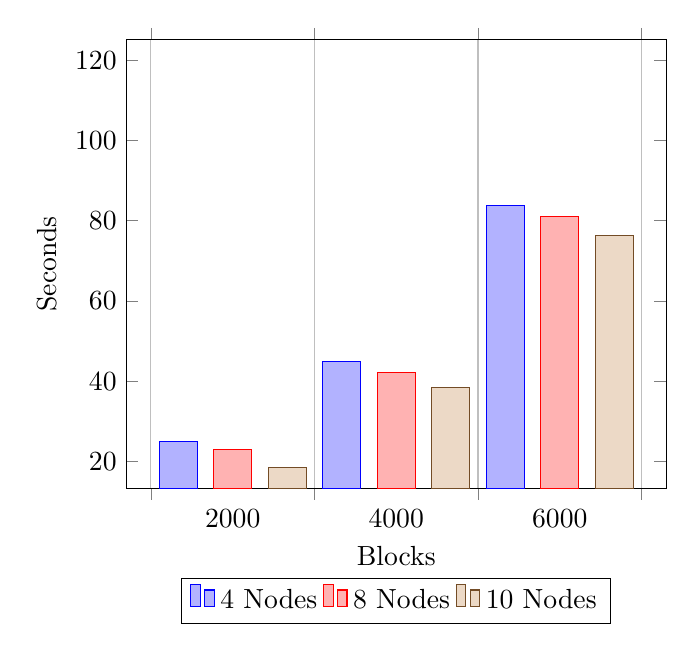
\begin{tikzpicture}
\begin{axis}[
	x tick label style={
		/pgf/number format/1000 sep=},
	ylabel=Seconds,
	xlabel = Blocks,
	enlargelimits=0.05,
	legend style={at={(0.5,-0.2)},
	anchor=north,legend columns=-1},
	ybar interval=0.7,
]
\addplot 
	coordinates {(2000,25) (4000,45)
		 (6000,83.8) (8000,120)};
\addplot 
	coordinates {(2000,23) (4000,42.1)
		 (6000,81) (8000,110)};
\addplot 
	coordinates {(2000,18.5) (4000,38.43)
		 (6000,76.25) (8000,106)};
\legend{4 Nodes, 8 Nodes, 10 Nodes}
\end{axis}
\end{tikzpicture}

\subsection{Power Consumption}
Using the power consumption variable, we want to note that since our algorithm uses a slightly more power efficient proof-of-work mechnism the amount of energy used by our mobile devices network is considerably reduced against the other studied approaches.

This is because the hashing mechanism to validate the blocks integrity use the bizantine agreeement factor similar to the expained in \cite{giladhemomicalivlachoszeldovich2017}.

The power consumption results matrix used by the network can be verified by this table:


\begin{table}[h!] 
\begin{center} 
\begin{tabular}{|l|c|c|c|}
%\begin{tabular}%{|m{2cm}|m{1.5cm}|m{1.5cm}|m{1.5cm}|}
\hline 

\textbf{} & \textbf{4 Nodes} & \textbf{8 Nodes}  & \textbf{10 Nodes}  \\ 
\textbf{}& \textbf{2 K + 2S} & \textbf{4K + 4S} & \textbf{5K + 5S} \\
\hline 
Modeled Power (Watts)& 2,8 & 2,9 & 3,0\\ 
\hline 
Measured Power (Watts) & 2,51 & 2,78 & 2,85\\ 
\hline
\end{tabular} 
\end{center} 
\caption{Power Consumption of the Mobile Network} 
\end{table}

\section{Related Work}

In another similar work, Suankaewmanee et al. \cite{Suankaewmanee} studied the performance of a mobile commerce application using blockchain technology in terms of computation energy, time consumption, and memory utilization. They introduce a mobile-commerce application using blockchain technology, the name was MobiChain, used for secured transaction. They develop an API which allows the mining process to be performed on mobile devices effectively.

Also, in \cite{RyanCole} they describe approaches to modeling the energy consumption of both Proof of Work in Bitcoin and non-proof-of-work coins and associated consensus algorithms based on parameters including the size of the network, the number of messages sent per transaction, and the computing cost of such a consensus protocol.

The authors in \cite{RichardDennis} conducts a formal analysis of the newly proposed temporal "rolling" blockchain using the B language. It will examine the security principles of the proposed model and conduct an in-depth analysis of the results, which will be compared to the security principles of traditional blockchain networks. Their aim is to demonstrate that our proposed model is a possible replacement to the traditional blockchain, and is capable of solving the scalability issue without introducing any additional security issues into the core data structure. 

In \cite{Yang} the authors consider an edge computing enabled mobile blockchain network, where IoT devices or mobile users can access and utilize resources or computing services from an edge computing service provider to support their blockchain applications. First, they present overviews of blockchain and edge computing architecture, respectively. They propose a prototype of an edge computing system for mobile blockchain. Then they propose pricing schemes for the edge computing services for mobile blockchain.



\section{Future Work}

Arguably the most important piece of work to conduct in the future is to make this proposed algorithm live, running on a complete market with thousands of transactions per day in a single or multiple devices. This will then let us examine in greater detail whether the assumptions in this paper hold true against a real world adversary, who controls various percentages of the network and other variables that may affect the obtained results.

The deployment onto a real world transactions network would also allow us to see whether our solutions to known issues and limitations hold true, or if new issues surface. It would also allow more research into possible secutiry vectors, such as an offline or online Internet connections between several mobile devices generating movements on the block chain.

Another key research area is implementing this algorithm, for example on a distrusted reputation network, to accurately model how the roll of the blockchain should be performed: i.e. whether a simple time period is sufficient, or if a more sophisticated model is required to allow millions of crypto or normal currency transactions to be processed in mobile devices.

As a major barrier for large-scale IoT blockchains is the transaction time, future research could be conducted to find out how the size of blockchain networks impacts the transaction time and what trade-offs between the energy usage and the transaction time may be on large-scale blockchains.



\section{Conclusions}
As mentioned before our novel approach to brings a power efficient and high performance blockchain implementation for mobile devices and it could be an useful platform to integrate secure transactions like e-commerce and currency exchange among heterogeneous network of mobile users without the requirement of external centralized validation.

The security of a blockchain system is given by the difficulty to be hacked and overrun by malicious participants to introduce fraudulent blocks to the transactions history. Since our algorithm actually ensures the participants should be able to make transactions with a high confidence of honesty between peers, we think that this will be the standard of future mobile trading and transactional exchanges by the blockchain method.

%\section{Conclusion}
%The conclusion goes here.





% if have a single appendix:
%\appendix[Proof of the Zonklar Equations]
% or
%\appendix  % for no appendix heading
% do not use \section anymore after \appendix, only \section*
% is possibly needed

% use appendices with more than one appendix
% then use \section to start each appendix
% you must declare a \section before using any
% \subsection or using \label (\appendices by itself
% starts a section numbered zero.)
%


%\appendices
%\section{Proof of the First Zonklar Equation}
%Appendix one text goes here.

% you can choose not to have a title for an appendix
% if you want by leaving the argument blank
%\section{}
%Appendix two text goes here.


% use section* for acknowledgment
%\section*{Acknowledgment}


%The authors would like to thank...


% Can use something like this to put references on a page
% by themselves when using endfloat and the captionsoff option.
\ifCLASSOPTIONcaptionsoff
  \newpage
\fi



% trigger a \newpage just before the given reference
% number - used to balance the columns on the last page
% adjust value as needed - may need to be readjusted if
% the document is modified later
%\IEEEtriggeratref{8}
% The "triggered" command can be changed if desired:
%\IEEEtriggercmd{\enlargethispage{-5in}}

% references section

% can use a bibliography generated by BibTeX as a .bbl file
% BibTeX documentation can be easily obtained at:
% http://mirror.ctan.org/biblio/bibtex/contrib/doc/
% The IEEEtran BibTeX style support page is at:
% http://www.michaelshell.org/tex/ieeetran/bibtex/
\bibliographystyle{IEEEtran}
% argument is your BibTeX string definitions and bibliography database(s)
\bibliography{bibliography}



% that's all folks
\end{document}


